\section{Performance}

\subsection{Module testing}

Detailed quality assurance procedures were developed for testing the modules during assembly at Fermilab, reception tests at Jefferson Lab, tracker integration, and commissioning. At each stage the results were compared with previous measurements. Module performance was tested by calibration procedures. No significant correlated noise has been observed between the channels of the same chip, chips of the same module or closely placed modules. The measured average channel noise (see Fig.~\ref{fig:enc-chip}) is comparable with the estimated contributions of different noise sources. The gain dispersion measured on the channels is within the specs of the readout chip (see Fig.~\ref{fig:gain-chip}).

\begin{figure}[hbt] 
\centering 
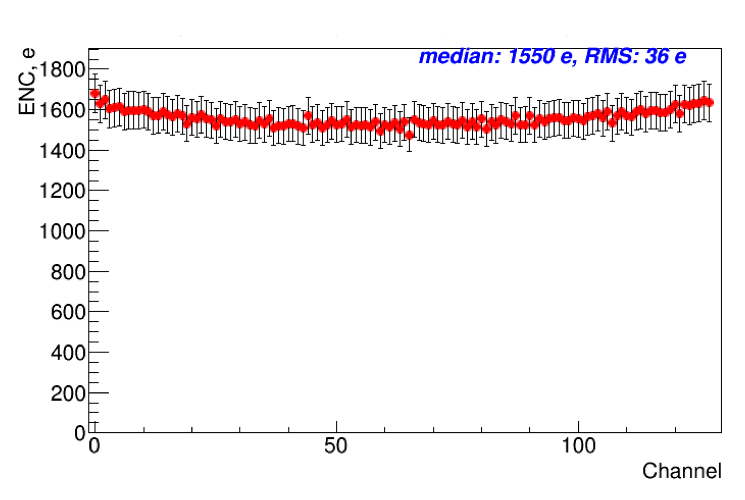
\includegraphics[width=0.8\columnwidth,keepaspectratio]{enc-chip.png}
\caption{Typical input noise on a single chip of an SVT module.}
\label{fig:enc-chip}
\end{figure} 

\begin{figure}[hbt] 
\centering 
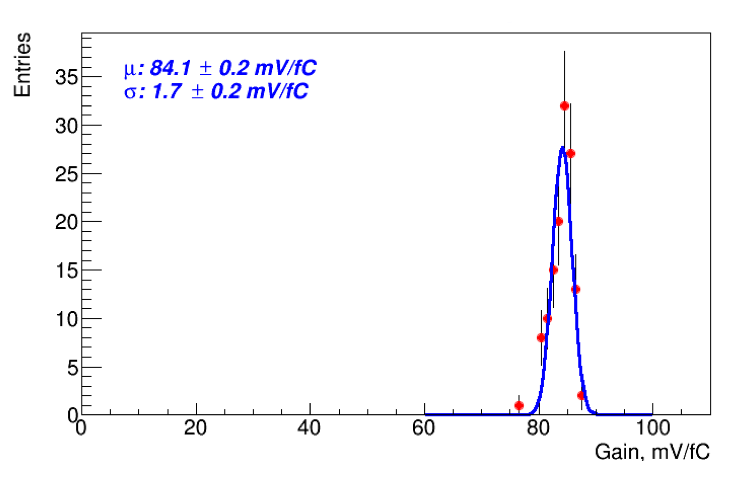
\includegraphics[width=0.8\columnwidth,keepaspectratio]{gain-chip.png}
\caption{Distribution of the gain for the channels of one representative FSSR2 ASIC.}
\label{fig:gain-chip}
\end{figure}

\begin{figure}[hbt] 
	\centering 
	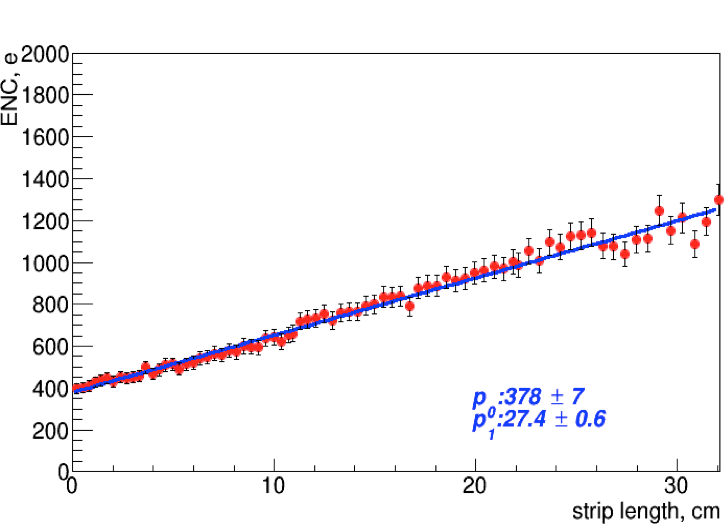
\includegraphics[width=0.8\columnwidth,keepaspectratio]{encstriplength.png}
	\caption{Input noise vs. strip length.}
	\label{fig:encstriplength}
\end{figure}

Longer silicon strips have higher capacitance and thus a higher input noise (see Fig.~\ref{fig:encstriplength}). Noise calibration accounts for the different strip lengths and pitch adapter layouts that affect the input capacitance of the preamplifier. The mean noise values scale linearly with strip length which confirms that the noise is dominated by the strip capacitance and not by coherent noise pickup of the system. The channel noise has a linear dependence on the strip length with the offset p$_{0}$ about 400 electrons corresponding to the ENC for the shortest strips and the slope p$_1$ of 27 electrons, consistent with expected FSSR2 noise performance at comparable capacitive load (see Fig.~\ref{fig:fssr2-enc-c}).

\begin{figure}[hbt] 
\centering 
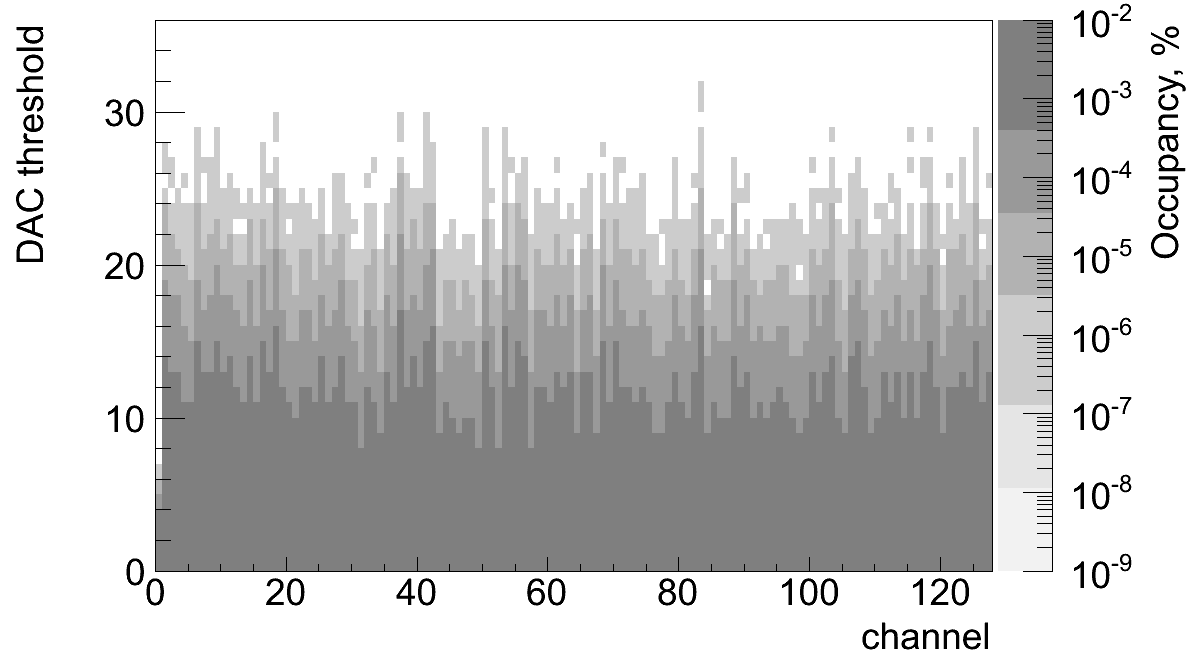
\includegraphics[width=0.8\columnwidth,keepaspectratio]{occ_thr.png}
\caption{Channel noise occupancy vs. DAC hit/no-hit threshold (in DAC bins, one DAC bin corresponds to 3.5~mV).}
\label{fig:noiseocc}
\end{figure}

The noise occupancy histogram with no charge injection is shown in Fig.~\ref{fig:noiseocc}. It probes the tail of the noise distribution, which can show effects masked by the higher occupancy at low thresholds. Channel noise allows setting a 3~$\sigma$ threshold at the 30~keV level. The Equivalent Noise Charge (ENC) of the SVT channels is shown in  Fig.~\ref{fig:enc}. The peak is $\sim$1600 electrons, the shoulder on the left side corresponds to the shorter strips. The channel noise allows setting a 3$\sigma$ threshold at the 20~keV level. 

\begin{figure}[hbt] 
	\centering 
	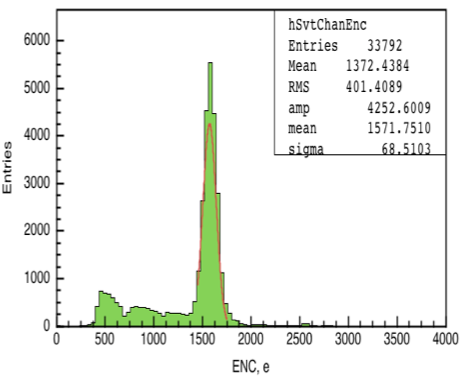
\includegraphics[width=0.8\columnwidth,keepaspectratio]{enc.png}
	\caption{SVT noise for all channels. The main peak corresponds to the full length strips (33 cm). The shoulder on the left side corresponds to the shorter strips.}
	\label{fig:enc}
\end{figure}

The detector response and full readout chain calibration was done with $\gamma$ and $\beta$ sources, cosmic muons, electron beam, and proton beam. The results of absolute gain calibration with a $\gamma$ source are shown in Fig.~\ref{fig:signal-gamma}. The signal peak is in good agreement with the expected position. The detector response to minimum ionizing particles was about 24000 electrons, which is what is expected for the 320 $\mu$m thick sensor.

\begin{figure}[hbt] 
	\centering 
	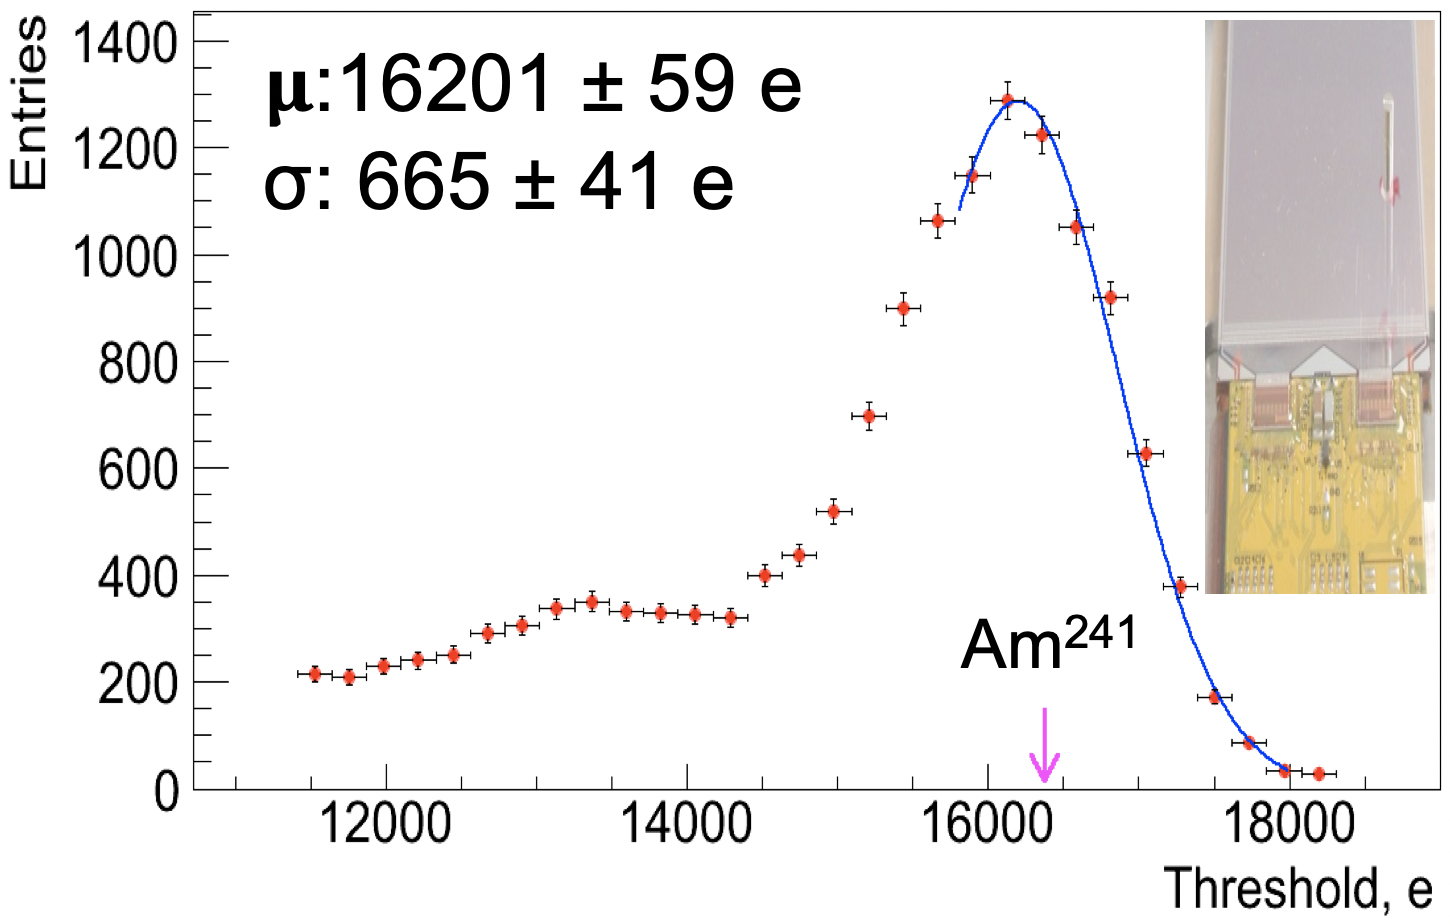
\includegraphics[width=0.8\columnwidth,keepaspectratio]{signal-gamma.png}
	\caption{Signal from Am$^{241}$ $\gamma$ source.}
	\label{fig:signal-gamma}
\end{figure}

%
%\begin{wrapfigure}{l}{0.5\columnwidth}
%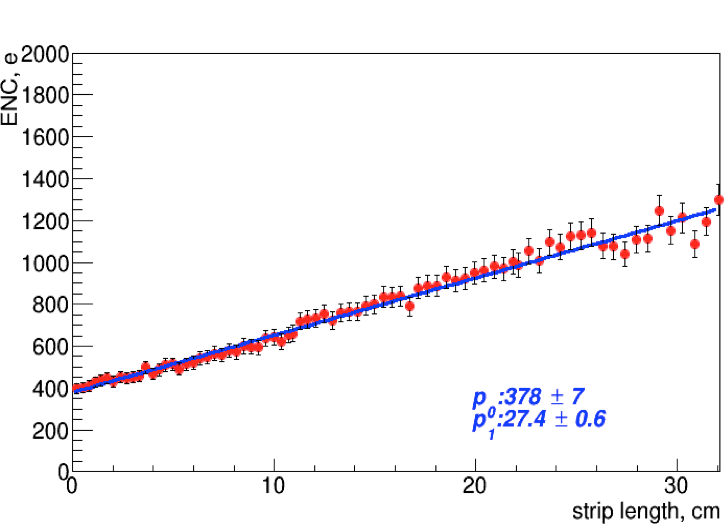
\includegraphics[width=1.0\columnwidth]{encstriplength.png}
%\caption{Input noise vs. strip length.}
%\label{fig:encstriplength}
%\end{wrapfigure}
%Longer silicon strips have higher capacitance and thus a higher expected value for the input noise. 
%(see Fig.~\ref{fig:encstriplength}).
%

%\begin{wrapfigure}{l}{0.5\columnwidth}
%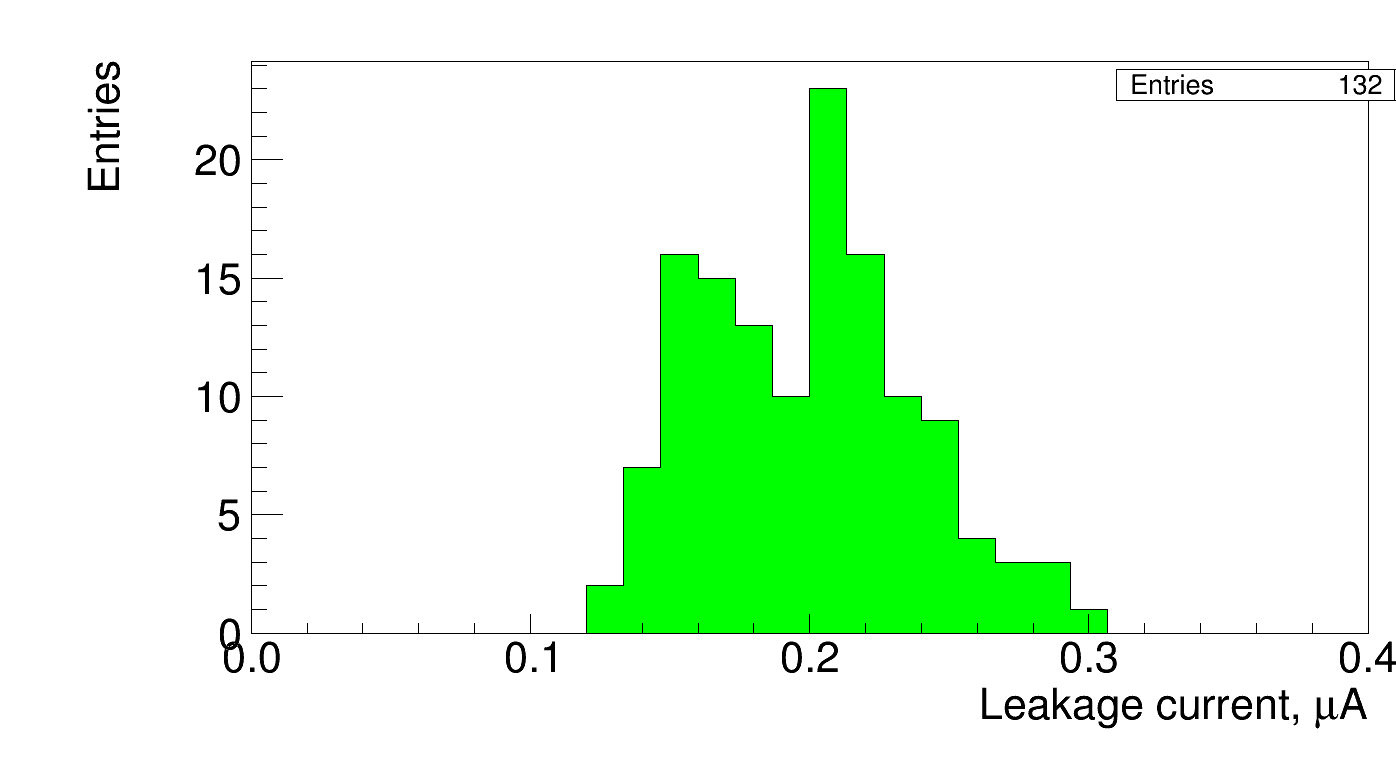
\includegraphics[width=1.0\columnwidth]{currents.png}
%\caption{Leakage currents}
%\label{fig:currents}
%\end{wrapfigure}
%
%\begin{wrapfigure}{l}{0.5\columnwidth}
%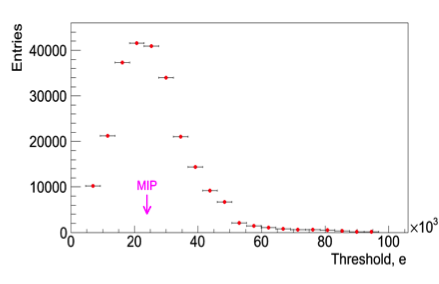
\includegraphics[width=1.0\columnwidth]{signal-muons.png}
%\caption{Signal muons}
%\label{fig:signal-muons}
%\end{wrapfigure}

\subsection{Integration and system checkout}

To verify performance of the integrated detector, data acquisition chain, power services, and cooling system, as well as the detector control and data acquisition software, the final detector system was installed in the clean room and used at all stages of tracker integration and commissioning. The SVT was operated for several months under environmental conditions close to the ones in the experimental hall. Defects known before the integration of the system were reestablished. 99.9$\%$ of channels were operational after the detector integration. 

\begin{figure}[hbt] 
\centering 
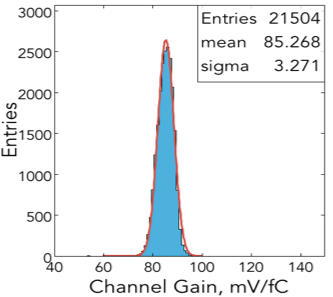
\includegraphics[width=0.6\columnwidth,keepaspectratio]{svt_gain.png}
\caption{Distribution of gain for the SVT channels.}
\label{fig:svt_gain}
\end{figure}

The noise behavior was found to be within expectations and well understood. The dependence of the noise on the environmental temperature and humidity is small. The noise performance in the experimental hall was comparable with the results taken in the clean room during integration. No significant correlated noise has been observed between the channels of the same chip, between the chips of the same module, or between the closely placed modules. The front-end electronics performed reliably, and no chip failures were observed. 
 
\begin{figure}[hbt] 
\centering 
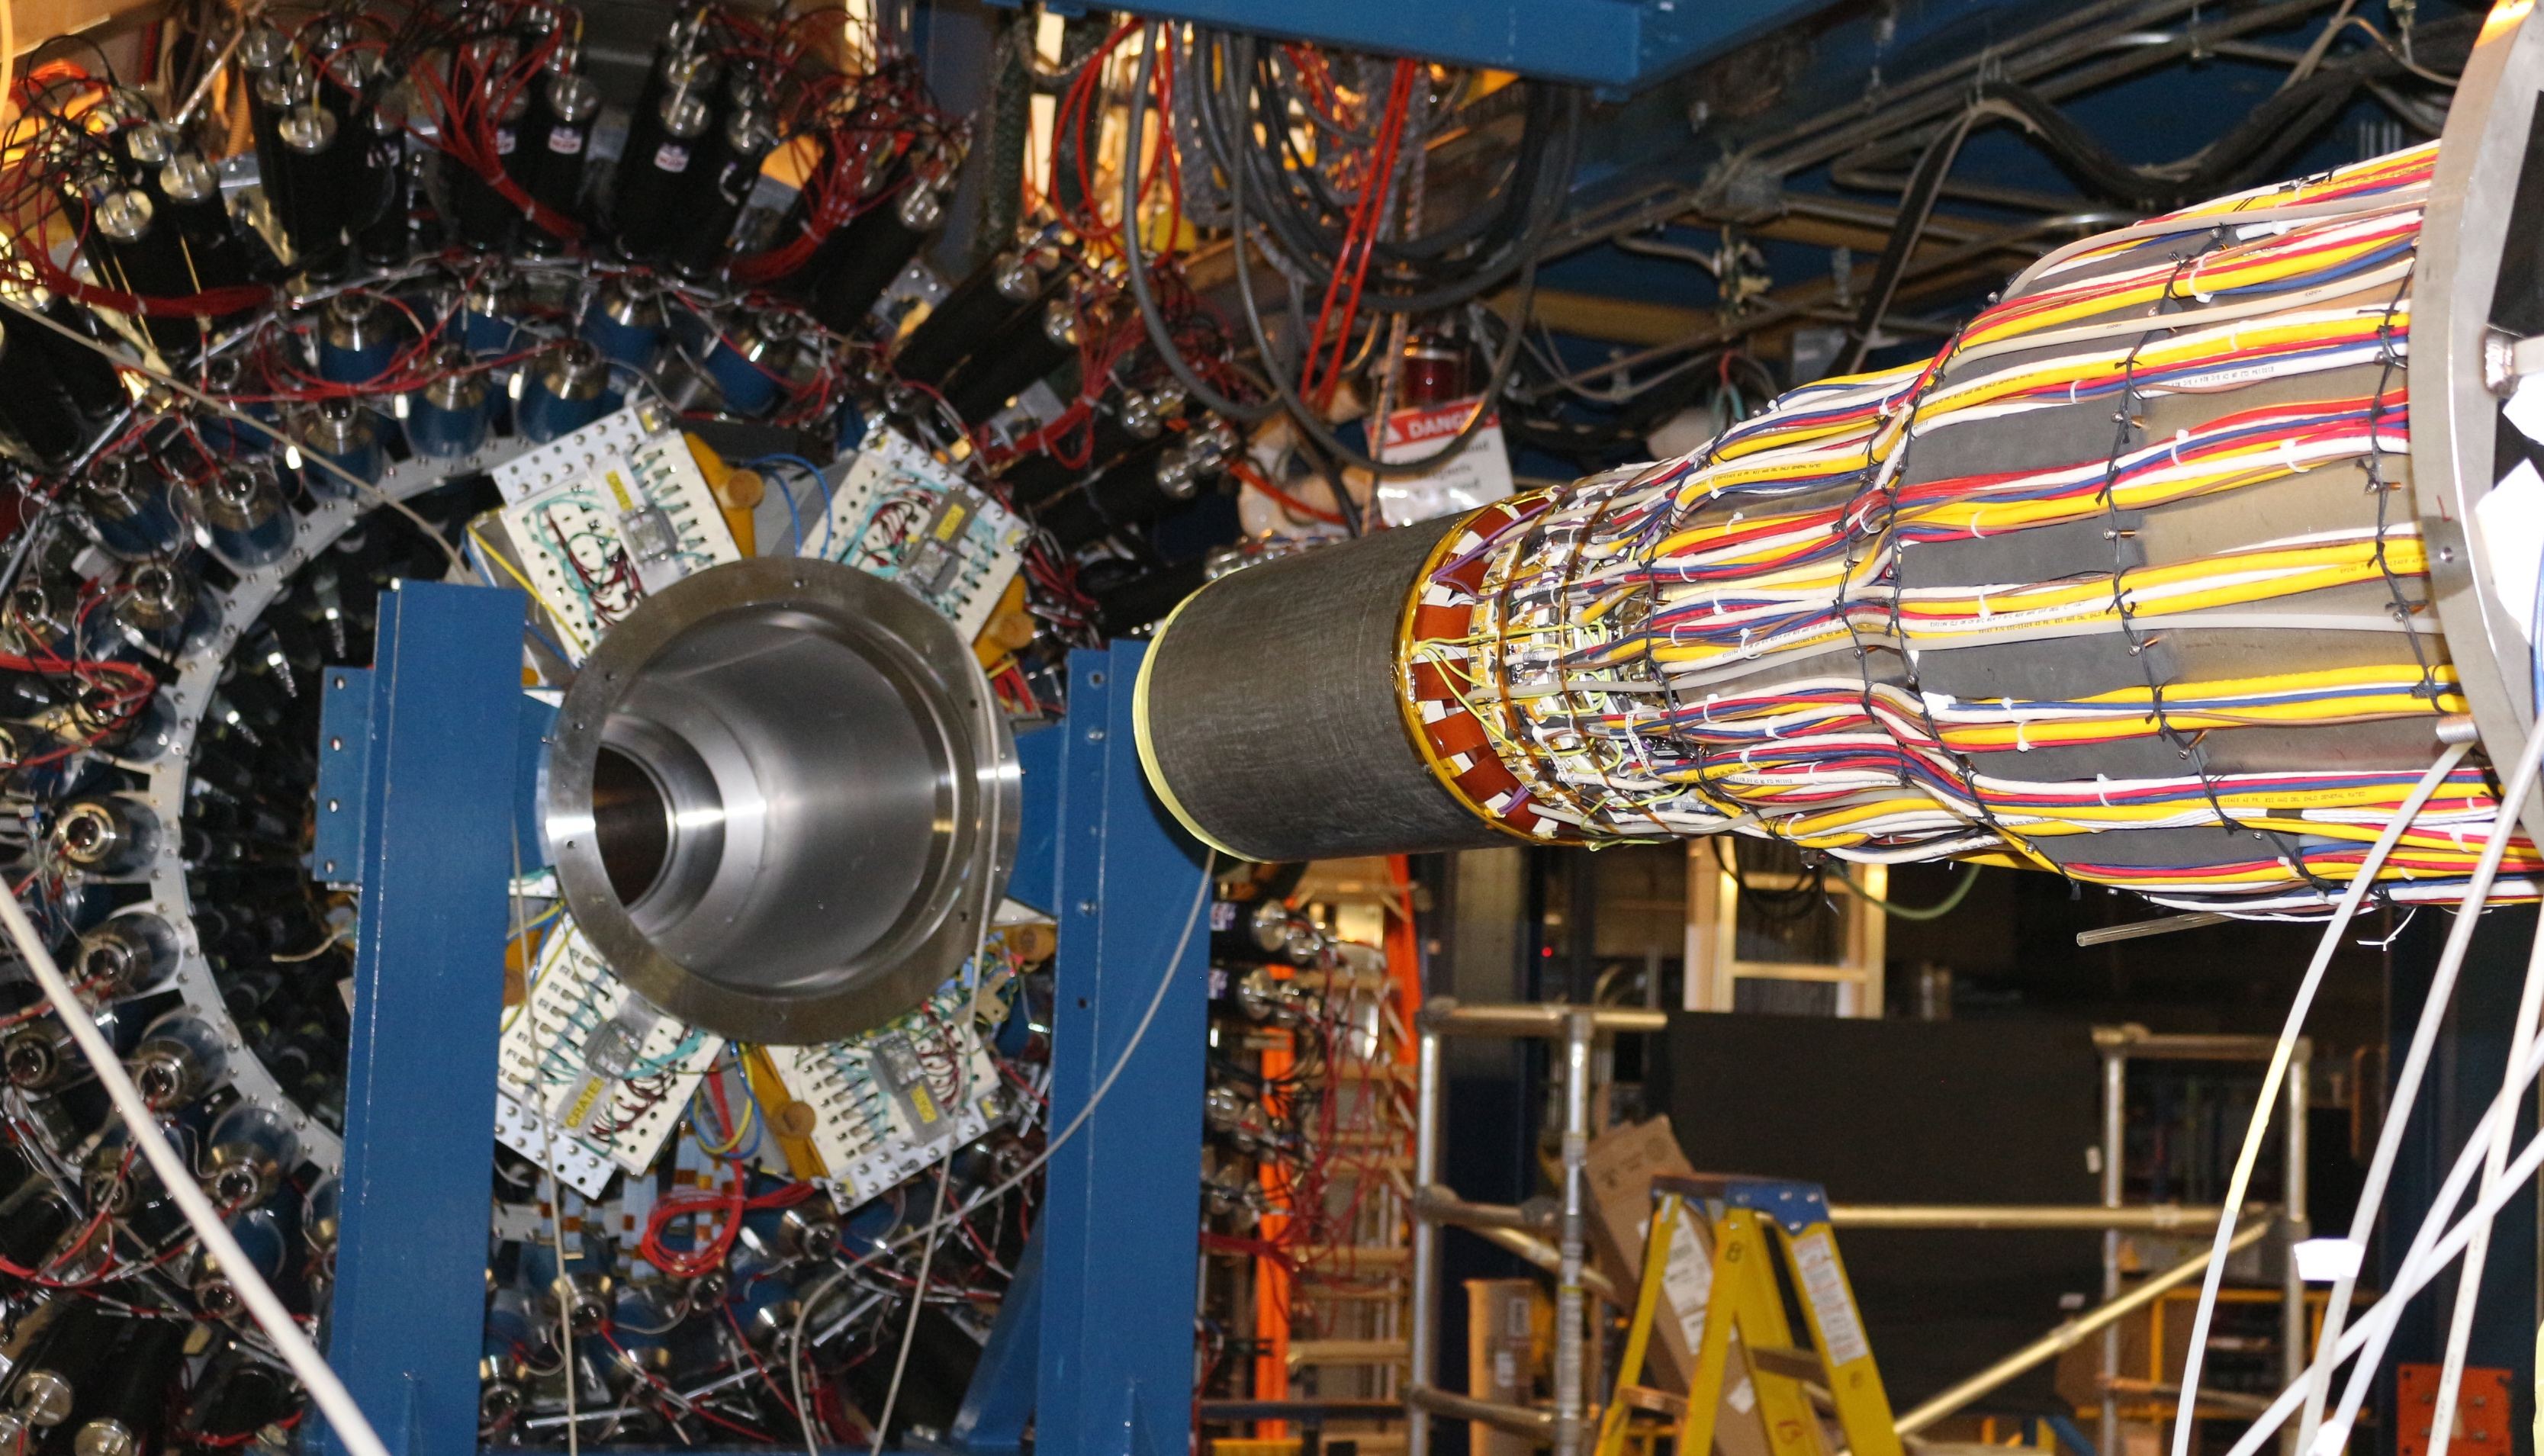
\includegraphics[width=0.8\columnwidth,keepaspectratio]{svt-hall.png}
\caption{SVT detector installed in the experimental hall before being pushed inside the CLAS12 detector.}
\label{fig:svt-hall}
\end{figure}

The distribution of gain was uniform and stable for all channels (see Fig.~\ref{fig:svt_gain}). All modules were found to be fully functional after transportation from the assembly site and installation on the beam line. Fig.~\ref{fig:svt-hall} shows the SVT detector after installation in the experimental hall.

\begin{figure}[hbt] 
\centering 
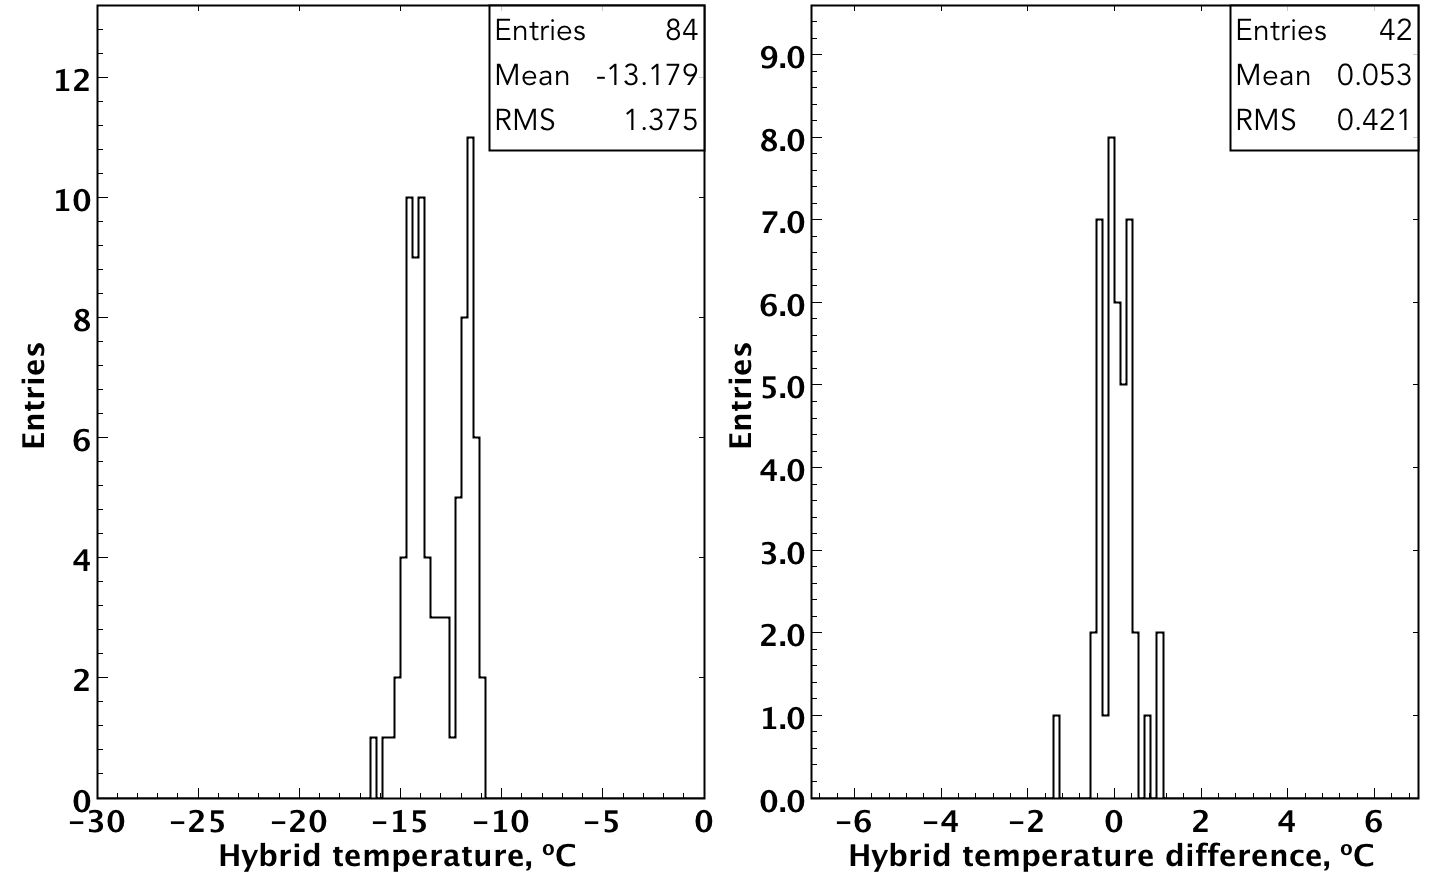
\includegraphics[width=0.8\columnwidth,keepaspectratio]{hybrid-temps.png}
\caption{Hybrid temperatures (left) and the difference in temperature between the two sides of the module with coolant at -26 $^\circ$C (right).}
\label{fig:hybrid-temps}
\end{figure}

Temperature variation of the SVT modules measured by sensors mounted on the hybrids with coolant at -26 $^\circ$C is shown in Fig.~\ref{fig:hybrid-temps} (left). In these operating conditions the module temperatures were uniformly distributed within the region, with lower temperatures close to the cooling lines. Region 3 temperatures were slightly higher than in the inner regions. The temperature difference between the two sides of a module is within 1$^\circ$C as shown in Fig.~\ref{fig:hybrid-temps} (right). Sensor leakage currents remained at the same low levels after installation (see Fig.~\ref{fig:currents}).

\begin{figure}[hbt] 
\centering 
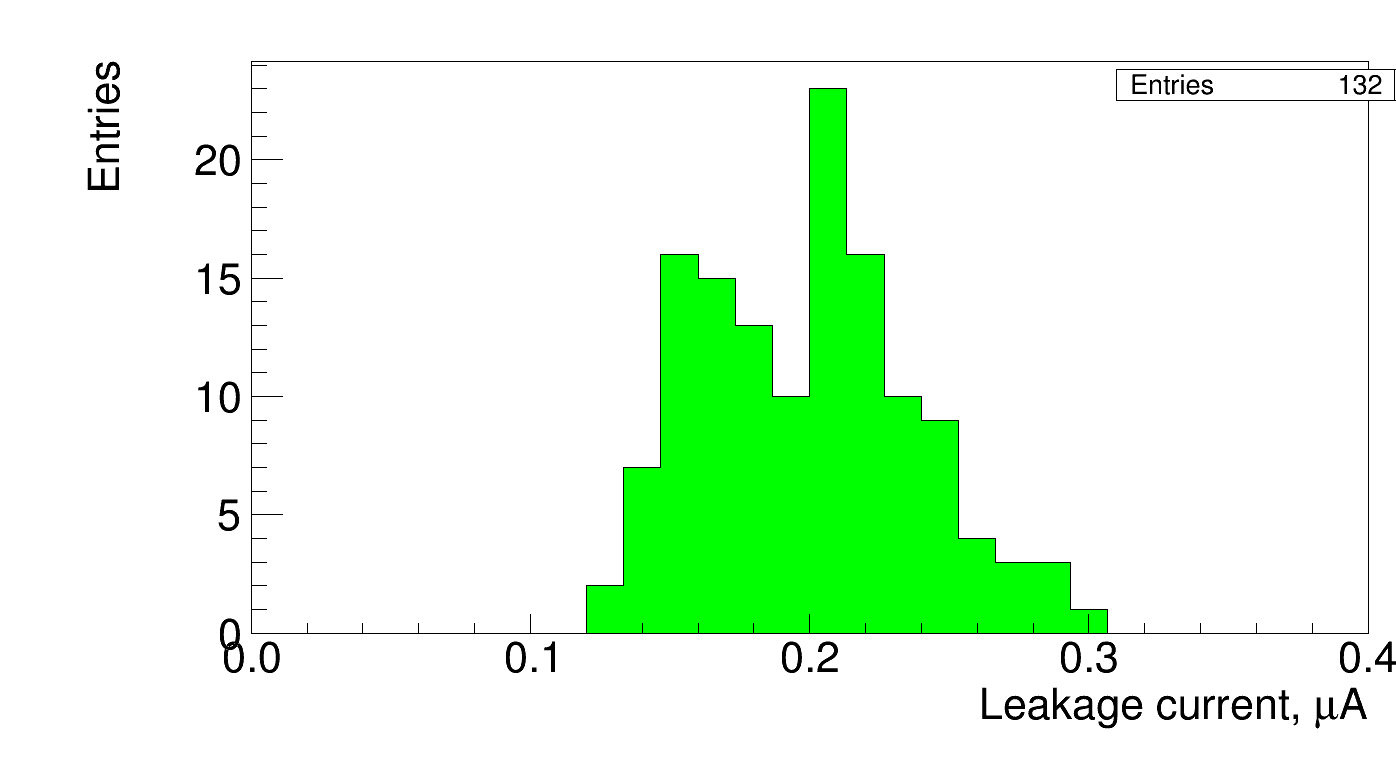
\includegraphics[width=0.8\columnwidth,keepaspectratio]{currents.png}
\caption{Sensor leakage currents after detector integration.}
\label{fig:currents}
\end{figure}

\subsection{Commissioning with cosmic rays}

Cosmic ray tests of the SVT have been used to test track reconstruction routines for the SVT, as well as to establish correct readout, good noise performance, and full response for the entire detector. Cosmic data during detector integration in the clean room were taken in the standalone mode using the self triggering feature of the FSSR2 readout chip in coincidence logic. VSCM boards reading the SVT modules located at the top and bottom halves of the horizontally placed barrel provided the trigger signals via signal distribution of two VXS crates. The coincidence of  signals from the trigger interface boards of both crates was taken as the cosmic trigger. 

After installation of the SVT in the hall, a trigger from CTOF detector was used to collect cosmic data for the CLAS12 central detector. A cosmic muon reconstructed in the central detector is shown in Fig.~\ref{fig:cd-cosmic-event}. Yellow circles represent crosses in the SVT and green circles correspond to the clusters in the Micromegas detector. A hit map for the SVT channels during the cosmic run is shown in Fig.~\ref{fig:cosmic-hitmap-svt}. The response of the channels was uniform, and performance results obtained during tracker integration were confirmed.
The angular distribution of the cosmic muons reconstructed in the SVT is shown in Fig.~\ref{fig:track-phi-theta}.

\begin{figure}[hbt] 
\centering 
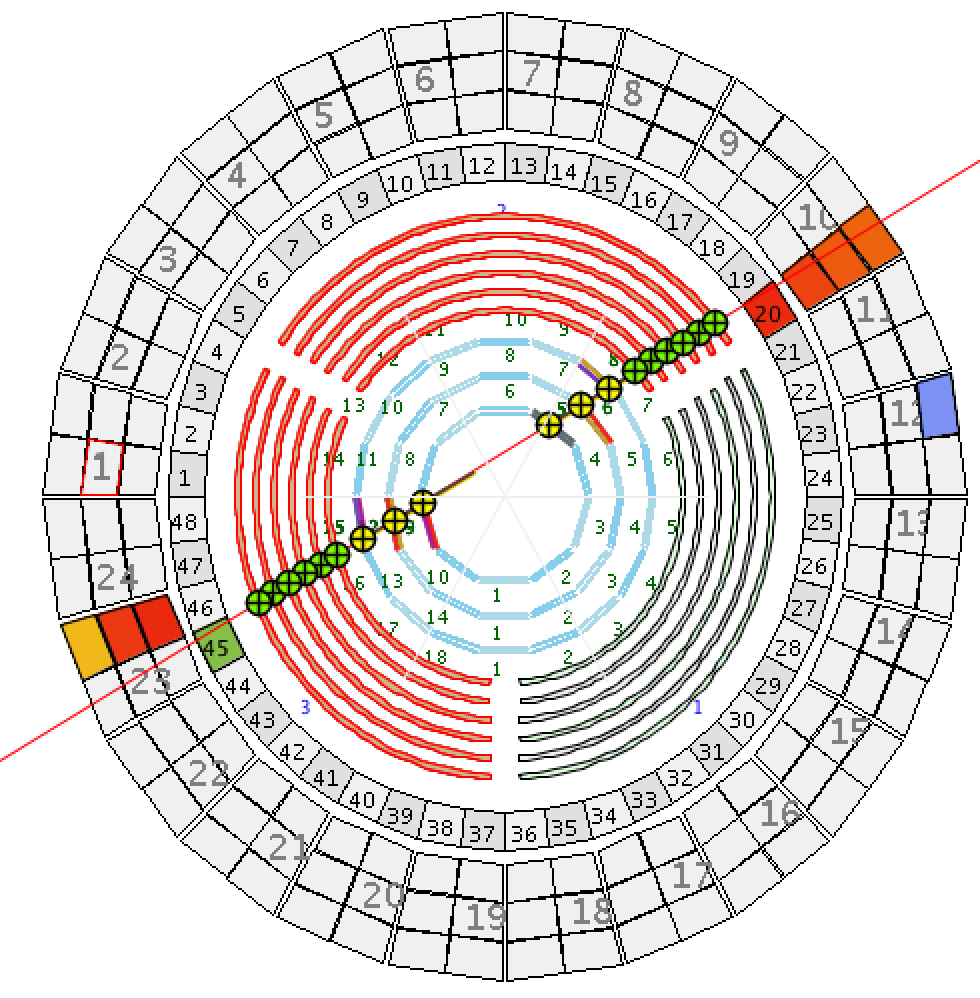
\includegraphics[width=0.6\columnwidth,keepaspectratio]{cd-cosmic-event.png}
\caption{Cosmic muon reconstructed in the CLAS central detector.}
\label{fig:cd-cosmic-event}
\end{figure}

\begin{figure}[hbt] 
\centering 
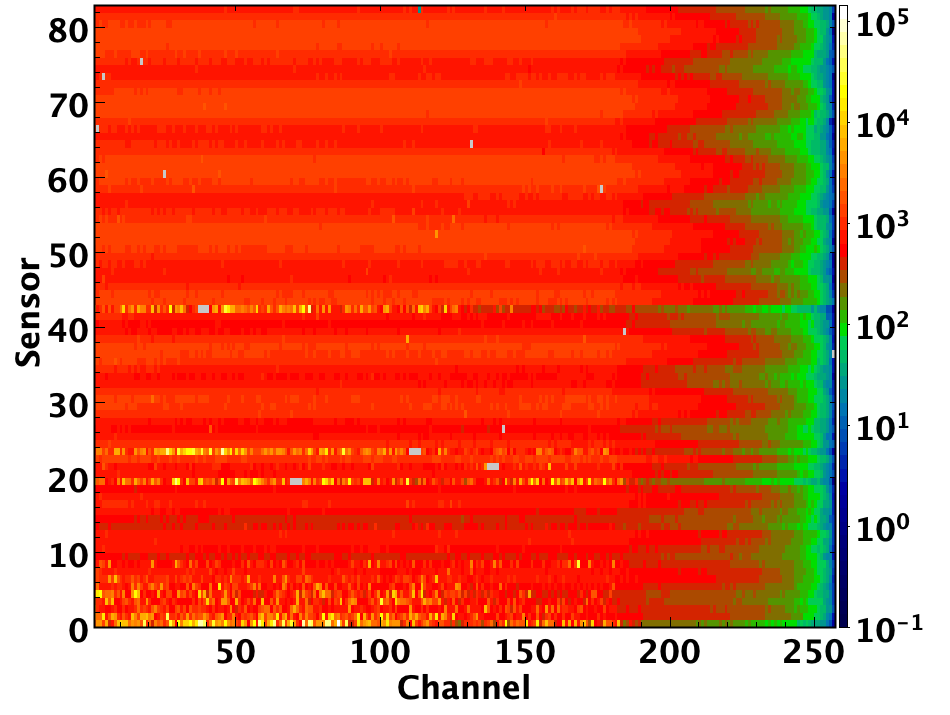
\includegraphics[width=0.8\columnwidth,keepaspectratio]{cosmic-hitmap-svt.png}
\caption{Monitoring SVT hit map during a cosmic run showing module vs. strip number.}
\label{fig:cosmic-hitmap-svt}
\end{figure}

A preliminary alignment of the SVT was done using the sample of the cosmic muon tracks taken without solenoid magnetic field. The spacial residuals before (blue) and after (red) the alignment procedure (see Fig.~\ref{fig:alignment}) are expected to provide the designed momentum resolution.

\begin{figure}[hbt] 
\centering 
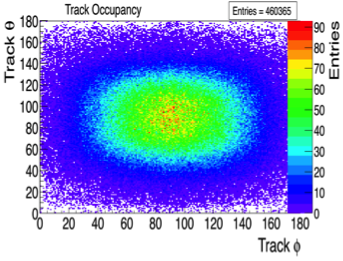
\includegraphics[width=0.8\columnwidth,keepaspectratio]{track-phi-theta.png}
\caption{Angular distribution of the cosmic muons reconstructed in the SVT.}
\label{fig:track-phi-theta}
\end{figure}

\begin{figure}[hbt] 
\centering 
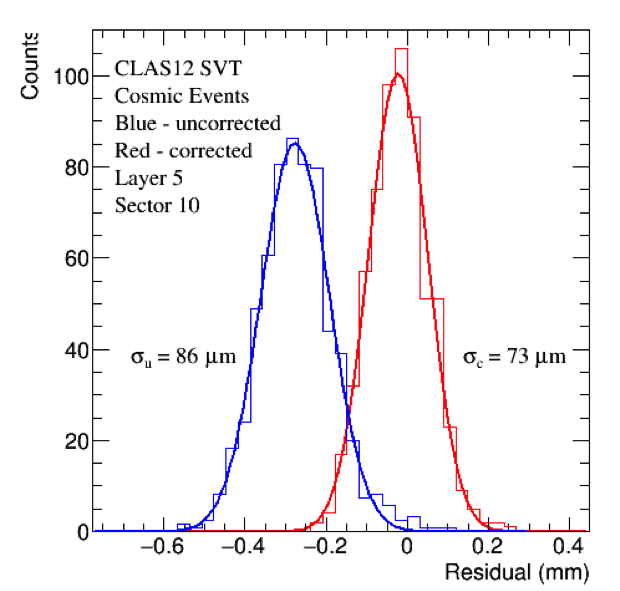
\includegraphics[width=0.6\columnwidth,keepaspectratio]{alignment.png}
\caption{Residuals for one of the SVT sensors before (blue) and after (red) alignment.}
\label{fig:alignment}
\end{figure}

\subsection{Commissioning with beam}

\begin{figure}[hbt] 
\centering 
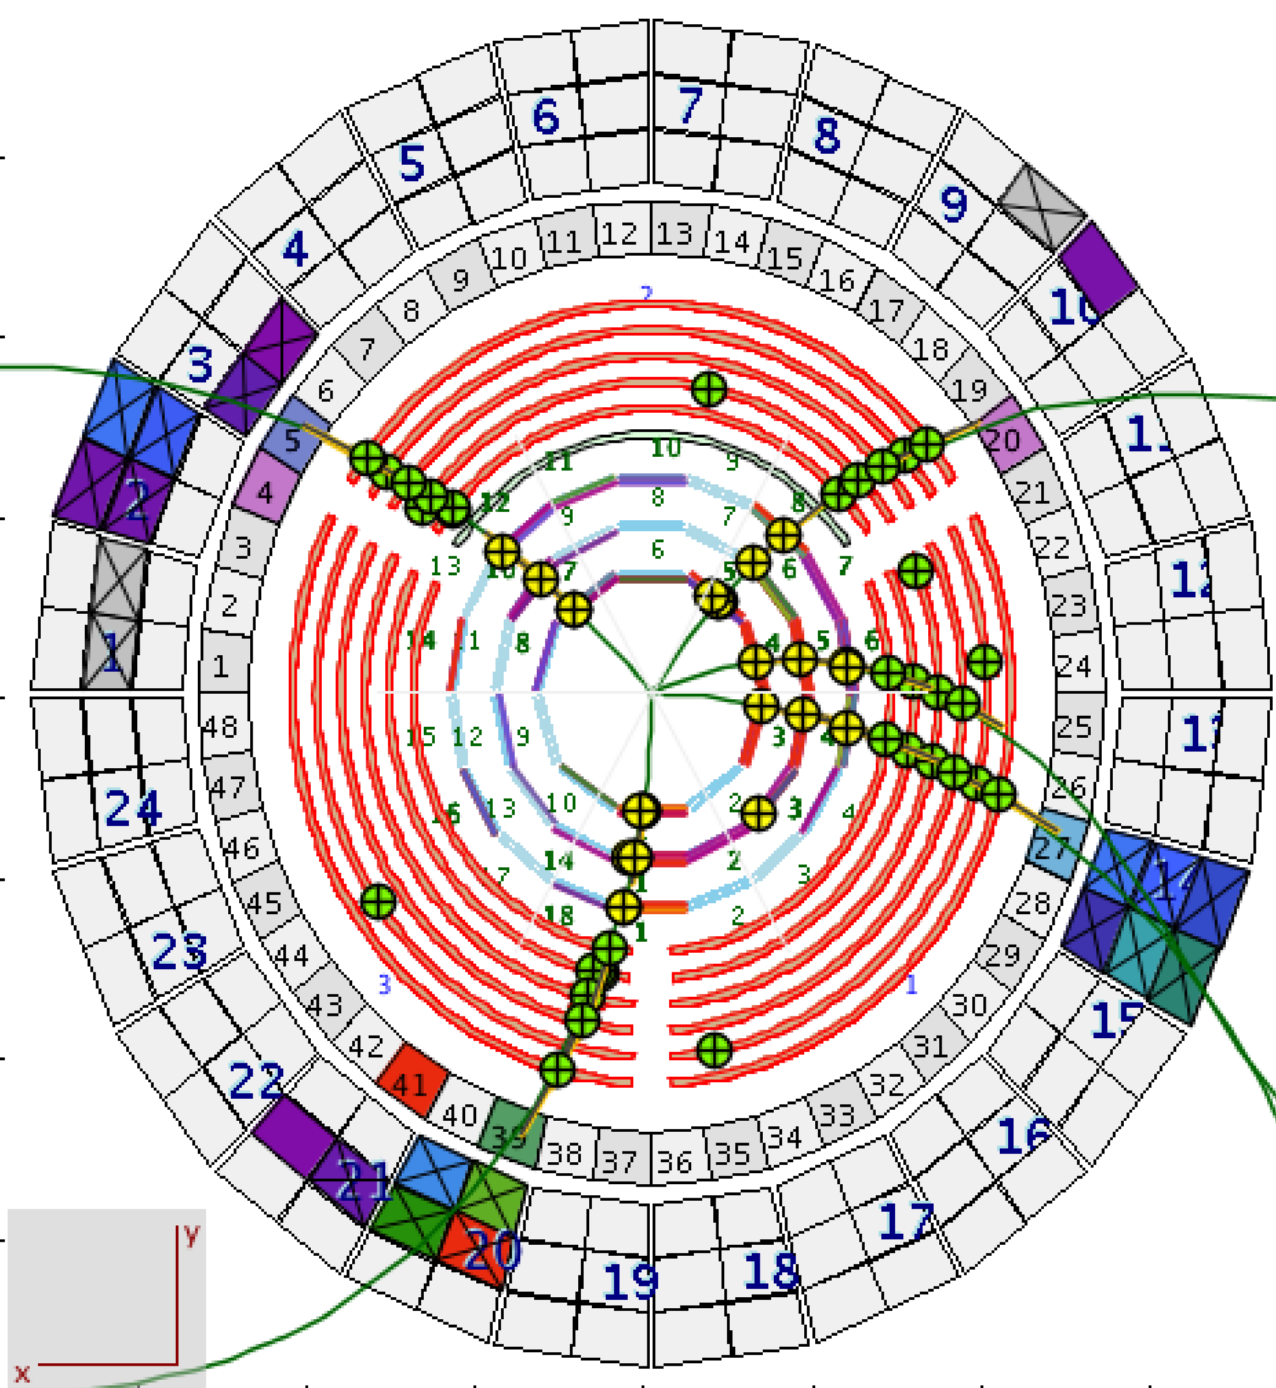
\includegraphics[width=0.6\columnwidth,keepaspectratio]{cd-tracks.png}
\caption{Multi-track event reconstructed in the CLAS12 central detector during a physics run.}
\label{fig:cd-tracks}
\end{figure}

The front-end electronics performance and noise occupancy of the detector were studied during physics data taking. No interference with other CLAS12 subsystems were found. The data quality and detector operational stability  were verified with both online and offline monitoring packages. There were occasional FSSR2 chip latch-ups observed after the start of a new run. These latch-ups were traced by improper configuration of the chips and fixed by adding additional resets to the run start sequence.

Tracks reconstructed in the CLAS12 central detector during a physics run are shown in Fig.~\ref{fig:cd-tracks}. The level-1 trigger latency is finely tuned to match the CLAS12 trigger delays.

\begin{figure}[hbt] 
\centering 
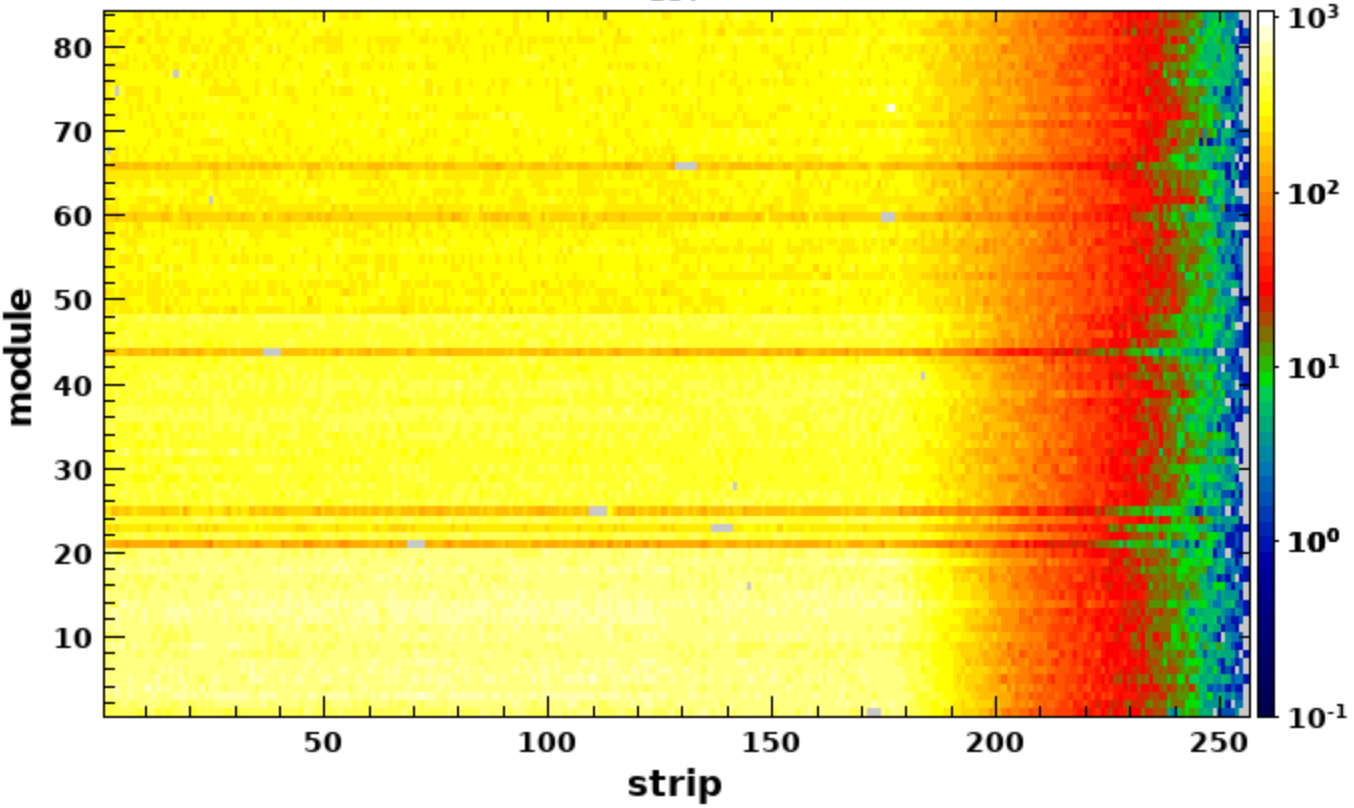
\includegraphics[width=0.8\columnwidth,keepaspectratio]{hit-map-rga.png}
\caption{SVT hit map during a physics run with the hydrogen target.}
\label{fig:hit-map-rga}
\end{figure}

After a year of running several sensors developed pinholes, observed as groups of adjacent hot channels. The bias voltage on these sensors has been lowered to reduce noise and abnormally high leakage currents. A hit map of the SVT from a physics run is shown in Fig.~\ref{fig:hit-map-rga}. Sensors with pinholes are seen on the map as darker horizontal lines due to lower efficiency with strips of masked hot channels. 

\begin{figure}[hbt] 
\centering 
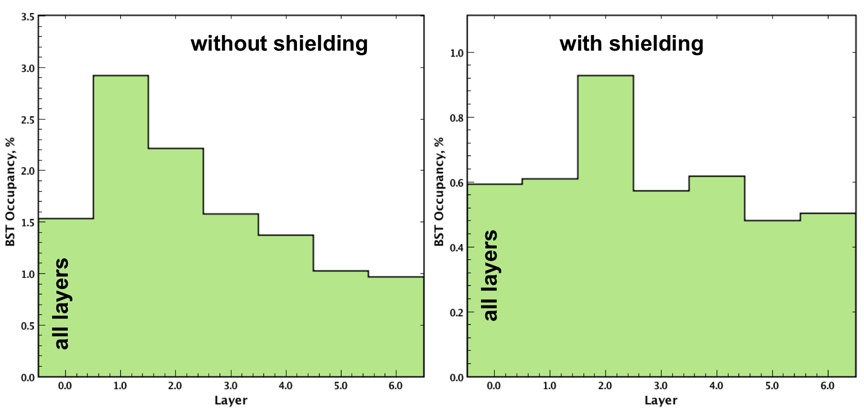
\includegraphics[width=0.8\columnwidth,keepaspectratio]{hit-occupancy-shielding.png}
\caption{Hit occupancies with and without the 50~$mu$m-thick tungsten shield installed outside of the target scattering chamber.}
\label{fig:hit-occupancy-shielding}
\end{figure}

The impact of the tungsten shield on the SVT occupancy is shown in Fig.~\ref{fig:hit-occupancy-shielding}. Occupancies in all SVT layers are substantially lower, which results in better tracking performance due to reduced combinatorics. The effect of the shield on the tracking performance is negligible~\cite{SHIELDNOTE}.


%\subsection{Tracking performance, resolution, efficiency}